\chapter{Results}
\label{chap:results}
In this chapter the results of the classification using “Max MCC” optimization strategy are presented. Some premises are necessary before proceeding with the interpretation of the data:
\begin{enumerate}
\item 	The average scores at the bottom of each table are between models with the same architecture, but different hyper-parameters. Furthermore, having an accuracy lower than the chance level but with a positive \ac{MCC} has been preferred compared to have the highest possible accuracy with a zero or negative \ac{MCC}.
\item 	CV Accuracy, CV Acc Std, \ac{CV MCC} and CV MCC Std stand for Cross-Validated Accuracy and MCC and their respective standard deviation.
\item 	Test accuracy and \ac{MCC} are computed using an unseen test split of the data. CV Accuracy and \ac{CV MCC} have been computed on the training split of the data; thus, their purpose is to provide a measure of consistency of the test scores (see Fig \ref{fig_data_split_strategy}).
\item 	The confidence interval has been calculated on the test split, Z=1.96. 
\item 	Chance level represents the default guessing of the majority class.
\item 	Standard deviation of each measure, if present, is between round parenthesis in the tables.
\end{enumerate}

First, the classification performances of \ac{SVM} and \ac{MLP} are compared for both arousal and valence classification. Then, the results are compared with related work.

\section{Support Vector Machines vs Multi-Layer Perceptron}
\label{sec:svm_mlp}
The results of the subject-dependent arousal classification experiment are reported in Table \ref{tbl:arousal_results}, while the results for valence classification are reported in Table \ref{tbl:valence_results}. In these tables, learning models can be identified by a positive \ac{MCC} score supported by a positive \ac{CV MCC} and are highlighted in blue. The models that over-fitted, highlighted in yellow, are characterized by negative \ac{MCC} and positive \ac{CV MCC}, meaning that they learned well on the training data but could not discriminate classes on the test data. Under-fitted models instead are characterized by zero or negative \ac{CV MCC} and positive or negative \ac{MCC}, because they did not have the adequate capabilities to capture the underlying structure of the training data, but possibly obtained a good test accuracy by random guessing and they are highlighted in orange.  In arousal classification the average majority class guessing (defined as chance level in the table) is \(58\pm8\%\), the highest and consistent test accuracy score is \(84\%\) with \ac{MCC} score of \(0.20\) using \ac{SVM} and \(88\%\) with \ac{MCC} score of \(0.78\) using \ac{MLP}. For \ac{SVM} classifiers, the average test accuracy is \( 61\pm9\%\) with average MCC of \(0.16\pm0.20\), \(61\pm6\% \) \ac{CV} accuracy and \ac{CV MCC} of \(0.24\pm0.12.\) For \ac{MLP} classifiers, the average test accuracy is \(58\pm12\%\), with average MCC of \(0.13\pm0.20\), \(57\pm8\% \) \ac{CV} accuracy and \ac{CV MCC} of \(0.15\pm0.16\). 

\begin{table}[h!]
  \caption{Arousal classification results using MCC as scoring parameter for GridSearch. Learning models are highlighted in blue, over-fitted and under-fitted models are highlighted in yellow and orange, respectively.}
  \label{tbl:arousal_results}
  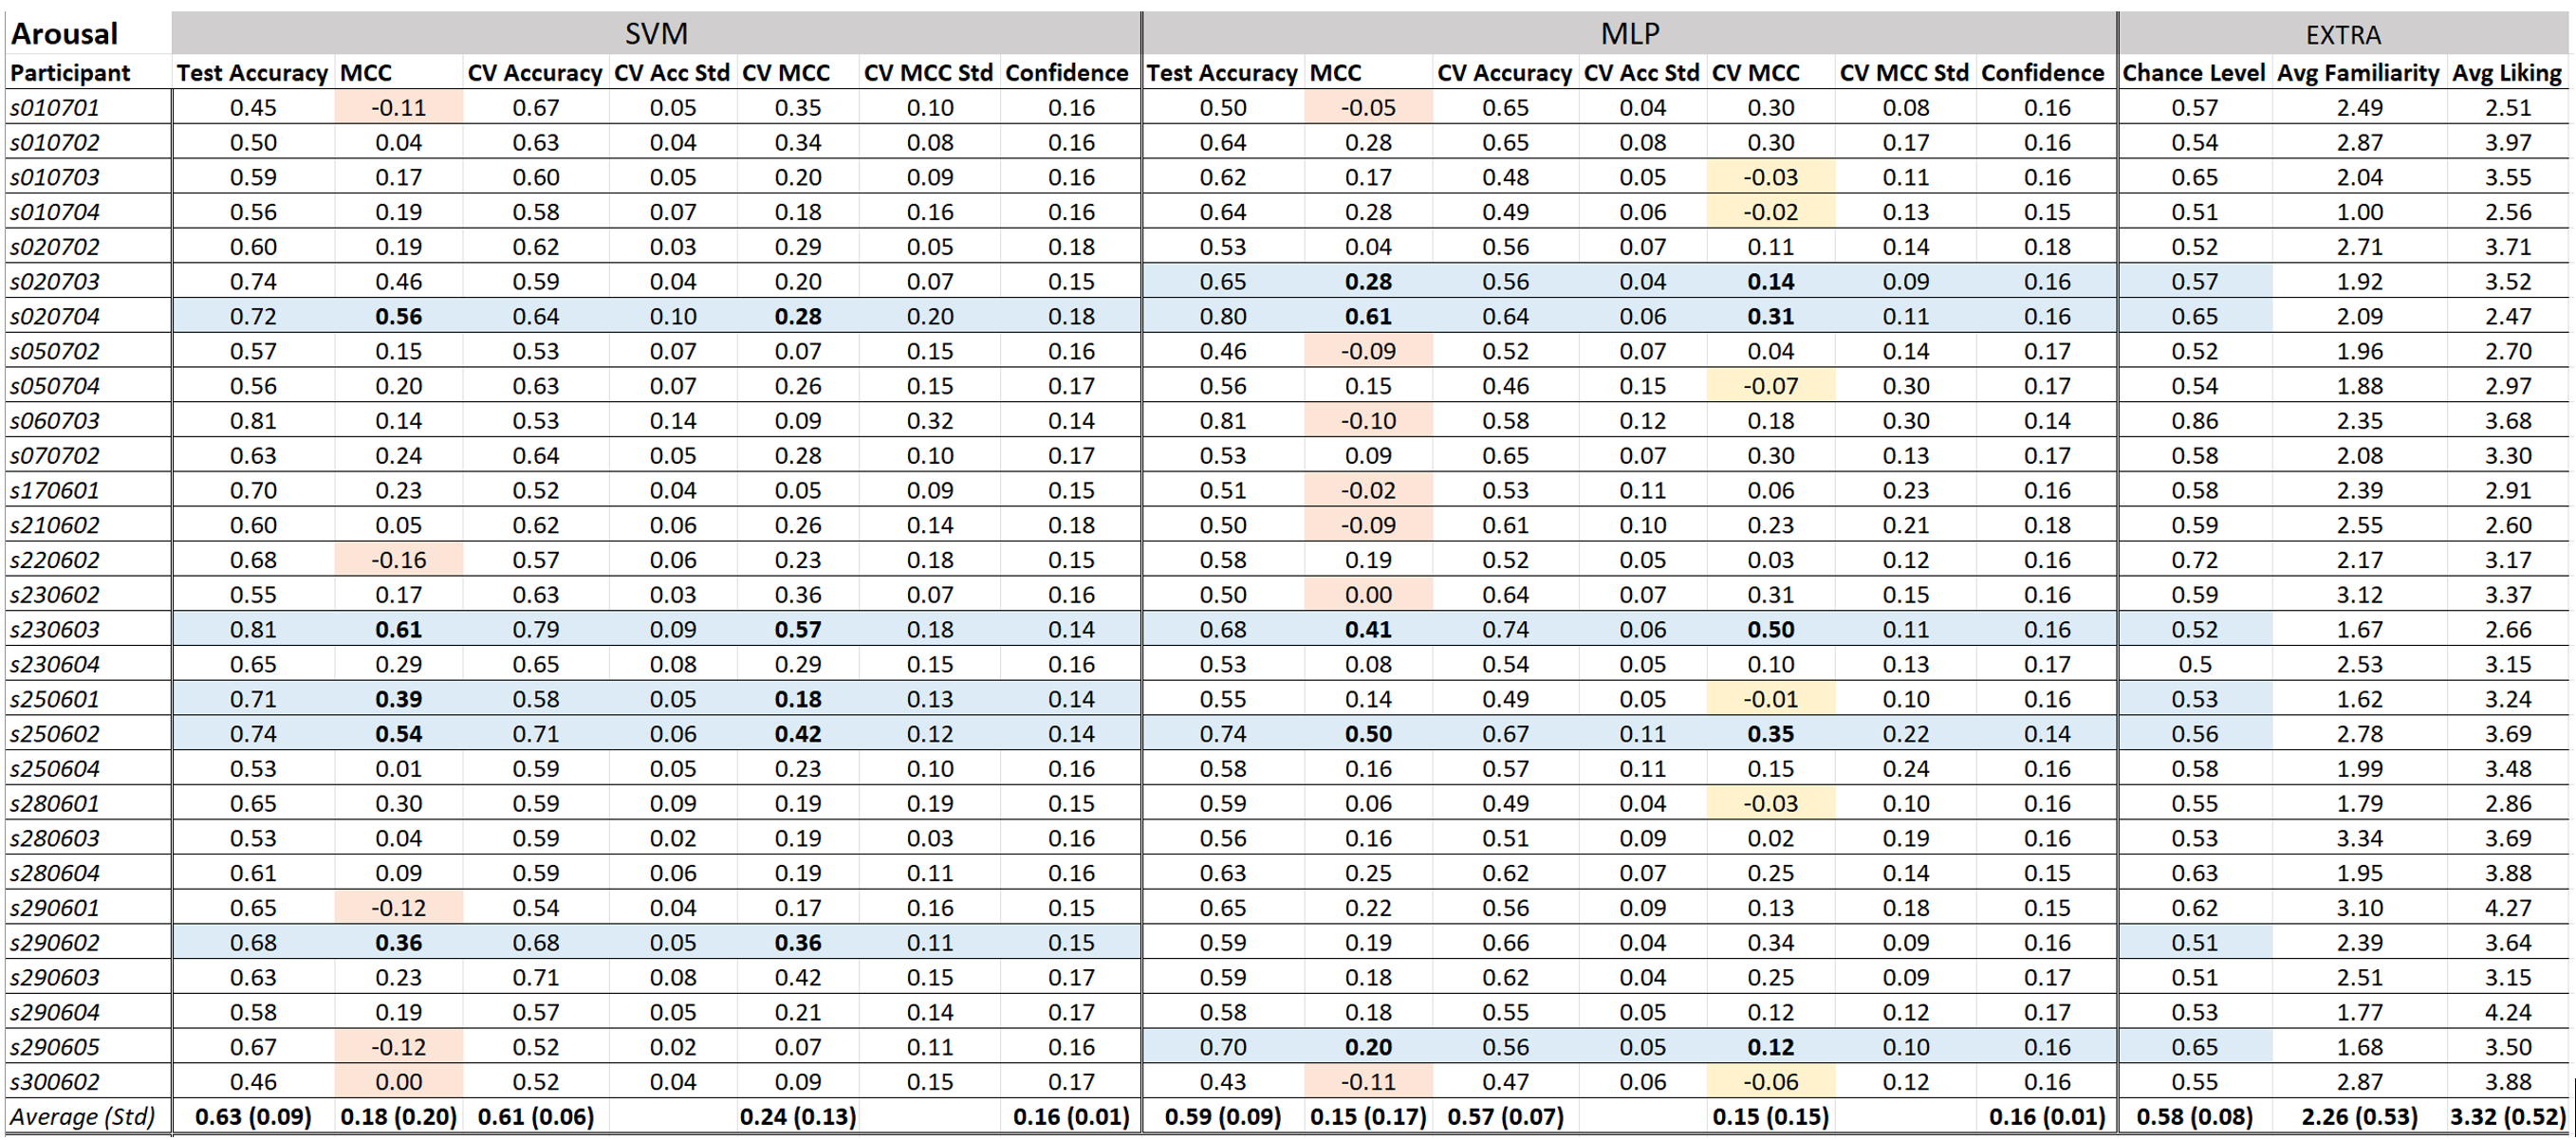
\includegraphics[width=\linewidth]{img/results/arousal_results.png}
\end{table}

In valence classification (see Table \ref{tbl:valence_results}) the average majority class guessing (defined as chance level in the table) is \(65\pm12\%\), the highest and consistent test accuracy score is \(89\%\) with \ac{MCC} score of \(0.27\) using \ac{SVM} and \(77\%\) with \ac{MCC} score of \(0.48\) using \ac{MLP}. For \ac{SVM} classifiers, the average test accuracy is \( 67\pm12\%\) with average MCC of \(0.13\pm0.18\), \(61\pm6\% \) \ac{CV} accuracy and \ac{CV MCC} of \(0.26\pm0.13.\) For \ac{MLP} classifiers, the average test accuracy is \(65\pm12\%\), with average MCC of \(0.11\pm0.18\), \(56\pm9\% \) \ac{CV} accuracy and \ac{CV MCC} of \(0.13\pm0.18\). The large variances are affected by the unbalanced distribution of positive and negative classes (see Chapter \ref{sec:unbalanced_labelling}), but it are also a clear symptom of diffused over-fitting, especially for \ac{MLP} classifiers. 

\begin{table}[h!]
  \caption{Valence classification results using MCC as scoring parameter for GridSearch. Learning models are highlighted in blue, over-fitted and under-fitted models are highlighted in yellow and orange, respectively.}
  \label{tbl:valence_results}
  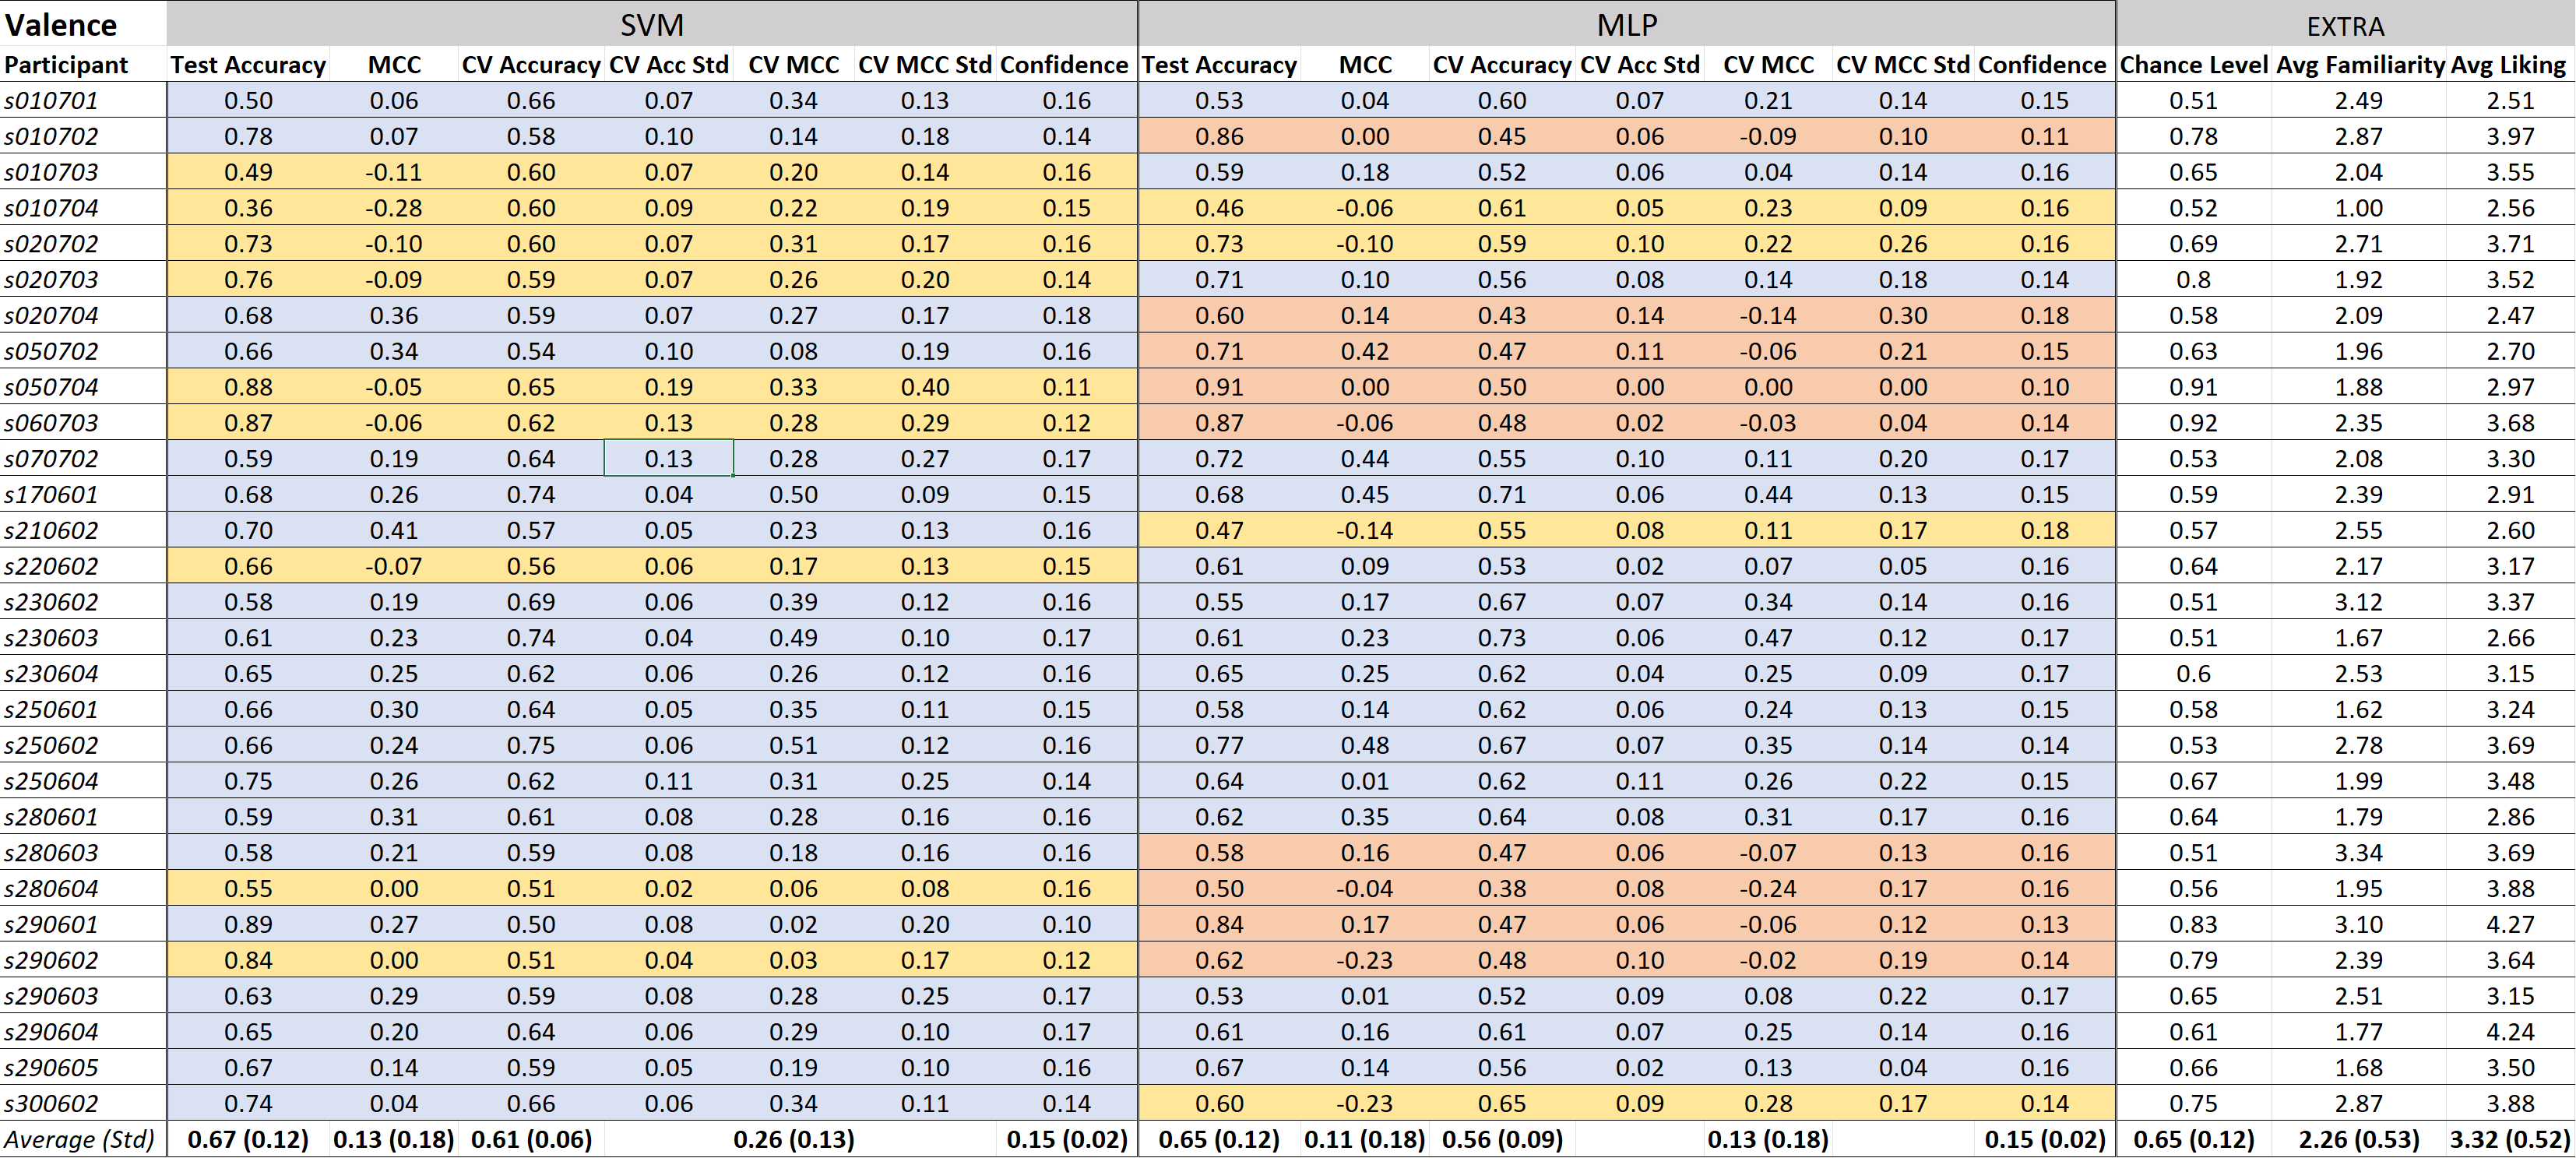
\includegraphics[width=\linewidth]{img/results/valence_results.png}
\end{table}

A final remark can be obtained by comparing the number of learning, over-fitting and under-fitting models between the two type of classifiers (see Fig. \ref{fig:svm_vs_mlp}. In arousal classification it was possible to train 25 \ac{SVM} learning classifiers, with 4 over-fitting models and 0 under-fitting models against 15 \ac{MLP} learning classifiers, 6 over-fitting models and 8 under-fitting models. In valence classification it was possible to train 20 \ac{SVM} learning classifiers, with 9 over-fitting models and 0 under-fitting models against 17 \ac{MLP} learning classifiers, 4 over-fitting models and 8 under-fitting models. 
Overall, the classification performances between \ac{SVM} and \ac{MLP} are not significantly different, but \ac{SVM} proved to be more reliable and obtained average classification accuracy above the majority default guessing threshold and generated more models able to discriminate unseen data. The are other model-specific advantages and disadvantages a to be taken into account in the implementation of a real-time application, for example most \ac{MLP} implementations support partial fitting of the models that is very useful with continuous streams of data, however these technical considerations lie outside the scope of this research.

\begin{figure}[h!]
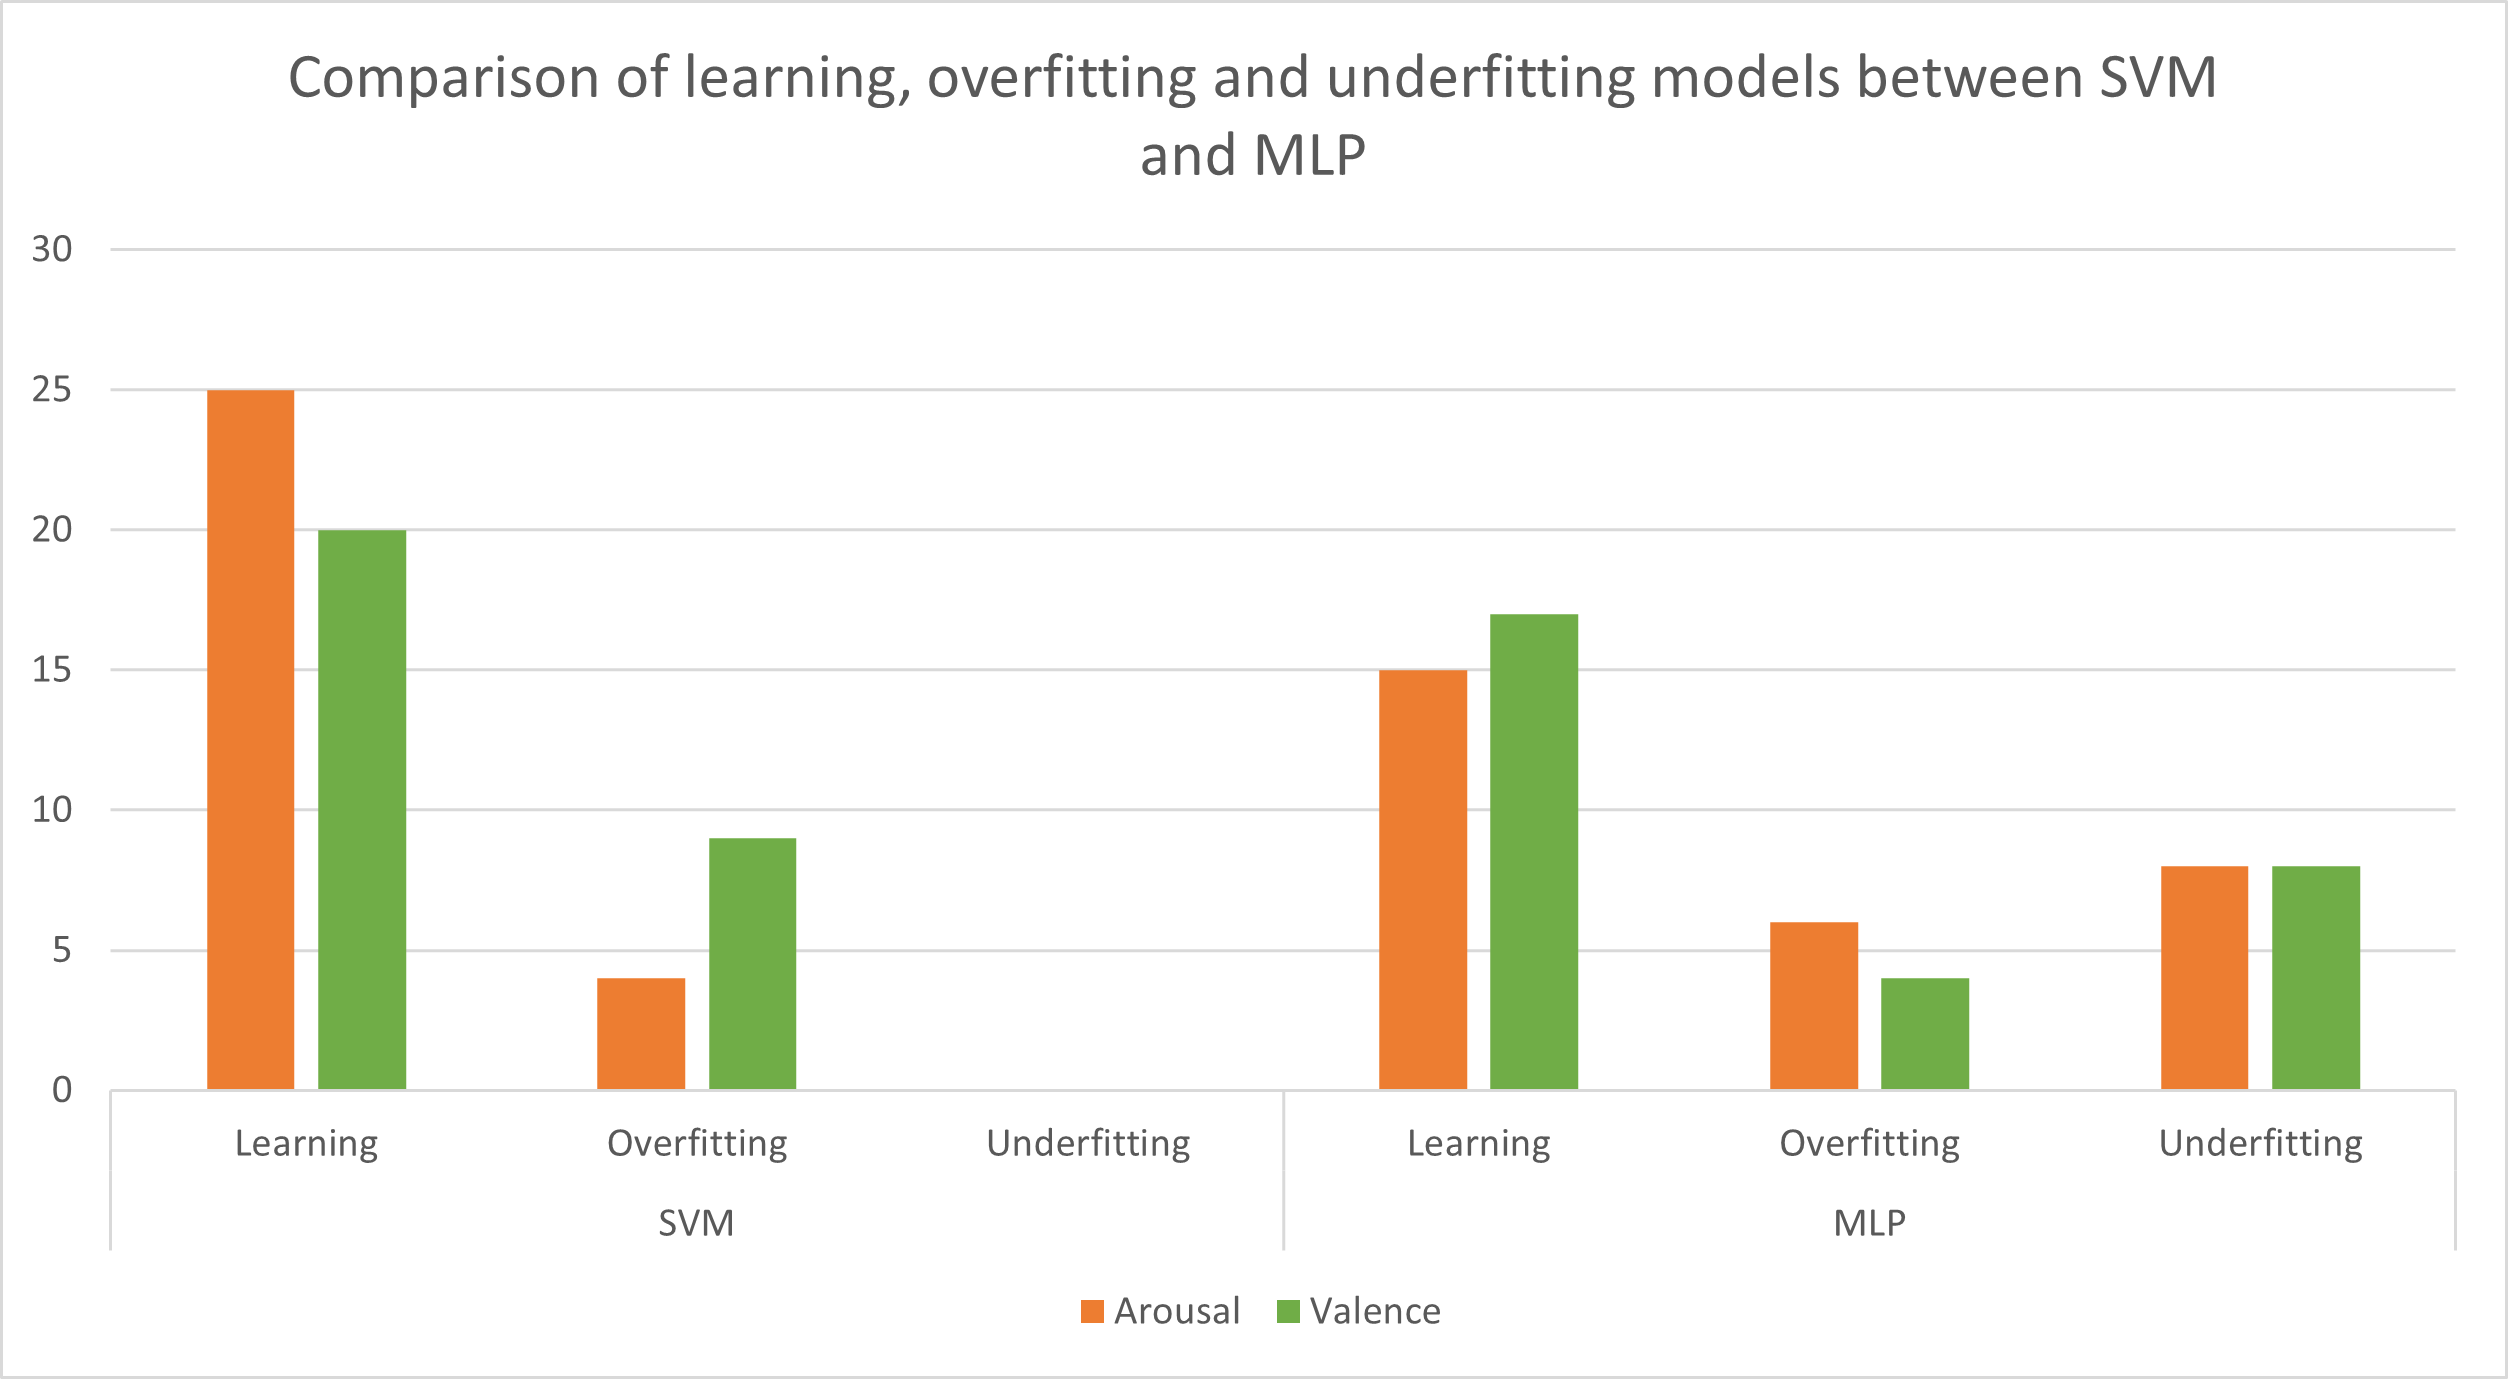
\includegraphics[width=12cm]{img/results/svm_vs_mlp.png}
\centering
\caption{Comparison of SVM and MLP in terms of number of learning, overfitting and underfitting models.} \label{fig:svm_vs_mlp}
\end{figure}



\section{Comparison with related work}
\label{sec:comparison}
Comparing the result of the current research with related work is non-trivial because of the methodological differences in data collection, processing, and evaluation. These differences have been considered to sort the comparisons from most comparable to least comparable. 
\\
The first and most comparable study \cite{thammasan_multimodal_2017} used self-reported continuous annotation as main labelling method for classification, the data were collected from 9 subjects with a wearable EEG headset equipped with 8 dry electrodes and processed using the automated PREP pipeline in MATLAB. The accuracy scores of SVM classifiers using EEG and LOBO cross-validation are only reported through plots, valence classification scored average accuracy of ~68\% and a standard deviation ~0.10, and arousal classification scored average accuracy ~64\% and a standard deviation ~0.10. The current study reports average test accuracy of 65\% (0.12) and average LOBO cross-validated accuracy on the training set of 61\% (0.07) for valence classification using SVM classifiers. Arousal classification scored an average test accuracy of 63\% (0.09) and average LOBO cross-validated accuracy of 61\% (0.06). They provided a table reporting the MCC scores for each classification modality, the average CV MCC reported for valence is 0.247 (0.17) and the average CV MCC for arousal is 0.177 (0.04). The current study reports average test MCC score of 0.10 (0.15) and average CV MCC score of 0.26 (0.15) for valence, while for arousal the average test MCC score is 0.18 (0.20) and average CV MCC score is 0.24 (0.13). Finally, the individual highest CV MCC score reported is 0.596 (0.3) for valence and 0.23 (0.22) for arousal, while in the current study the highest CV MCC score reported is 0.53 (0.13) for valence and 0.57 (0.18) for arousal, using SVM. These results are aligned with the current study and provide individual insights for each subject that can be easily compared.
\\
The second comparable study \cite{thammasan_continuous_2016} is the one that inspired the self-reporting of emotions using continuous annotation. The focus of this study, however, was to compare traditional discrete annotations to continuous annotation and to evaluate two approaches for features extraction. For comparison purposes, the scores reported using PSD features will be considered instead of the scores obtained with FD features. The accuracy scores, and relative standard deviations are mostly reported in plots and partially during the discussion, so an estimate is provided. Using SVM, valence classification score is ~81.2\% (0.08) average CV accuracy and arousal classification score is ~75\% (0.08) average CV accuracy. With MLP, valence classification score is ~80.2\% (0.1) average CV accuracy and arousal classification score is ~75\% (0.1) average CV accuracy. These scores are significantly higher than chance level and clearly outperform the results obtained in the current study, that are not on average significantly higher than chance level. No further insights are provided on individual performances, so they can be considered not relevant. 
\\
The third study \cite{wu_estimation_2017} aimed at artificially simulating a wearable device by selecting, 2, 4 and then 8 frontal electrodes from the subjects of the DEAP dataset, collected with and EEG system with 32 wet electrodes and discrete self-reported labels. Only the results for the 2 electrodes configuration using SVM for subject-dependent classification are reported and no specific description of the preprocessing pipeline is provided. The average CV accuracy scored for valence classification is ~68.4\% (0.02). The authors also provide better scoring using GBDT classifier for subject-dependent and subject-independent classification and a balancing strategy for the labels is explained, but no specific distribution of positive and negative class is provided, nor individual insights for subject-dependent classification.
\\
The fourth and last comparable study \cite{lin_eeg-based_2009} collected self-reported continuous annotations from 26 subjects using a standard EEG system with 32 wet electrodes. The data were preprocessed with visual inspection on EEG lab and then features were extracted from 12 pairs of symmetrical electrodes. The authors provide 3 classifications schemes, but only the “one-against-one scheme is comparable in terms of binary classification of valence and arousal and therefore reported. The reported CV accuracy score for valence classification is 94.86\% (0.176) and for arousal classification is 94.43\% (0.212). The authors did not report the distribution of the classes.
